\documentclass{article}
\usepackage[utf8]{inputenc}
\usepackage{amssymb,amsmath}
\usepackage[parfill]{parskip}
\DeclareMathOperator*{\argmin}{arg\,min}
\DeclareMathOperator*{\argmax}{arg\,max}
\usepackage{graphicx}
\usepackage{subcaption}

\usepackage{mathtools}
\DeclareMathOperator{\tr}{tr}

\title{Optimization 10/36-725\\
        Homework 2}
\author{Willie Neiswanger}
\date{}

\begin{document}

\maketitle


\section{Problem Three}

%\subsection{(a)}
\begin{figure}[h!tbp]
        \center{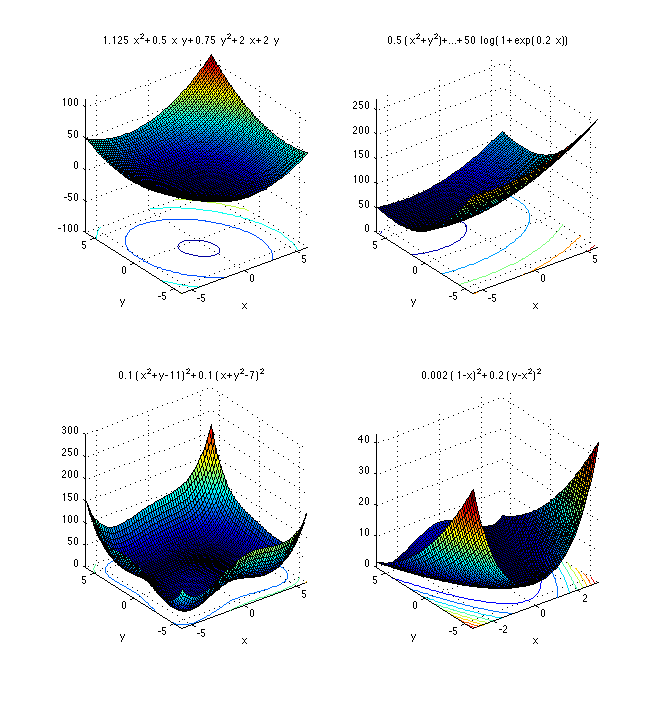
\includegraphics[width=0.6\textwidth]{img/surf.png}}
       \caption{Surface plots of the four functions: $f_Q$ (upper left),
       $f_{LL}$ (upper right), $f_H$ (bottom left), $f_R$ (bottom right).}
\end{figure}

%\subsection{(b)}

\begin{figure}[h!tbp]
        \center{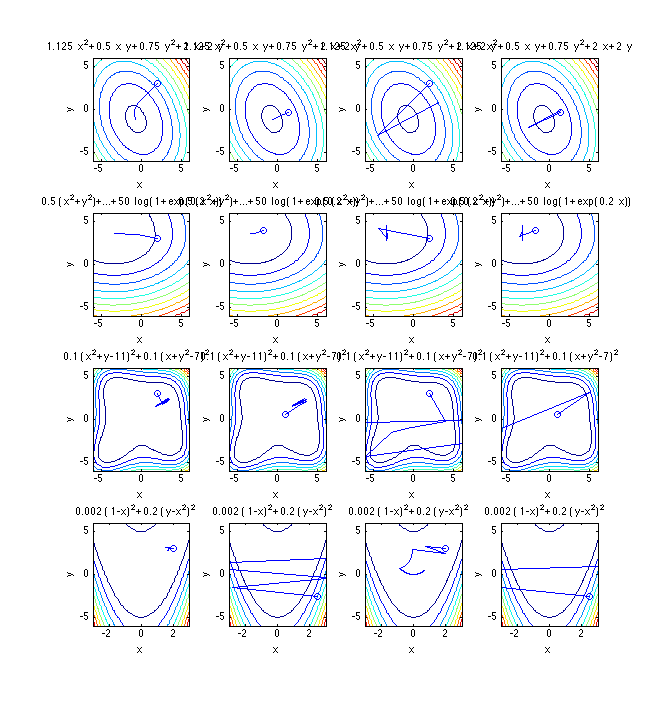
\includegraphics[width=1\textwidth]{img/gd_fixed.png}}
       \caption{Gradient descent with fixed step sizes: each row is a different
       function, the first two columns are with $0.3$ step size (fixed initialization,
       then random initialization), and the second two columns are with $0.8$ step size.}
\end{figure}

%\subsection{(c)}
\begin{figure}[h!tbp]
        \center{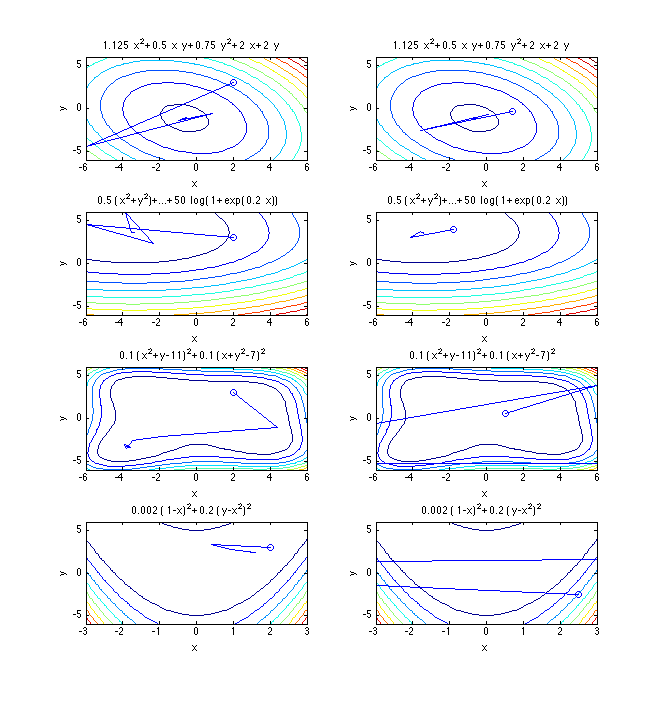
\includegraphics[width=1\textwidth]{img/gd_bt.png}}
       \caption{Gradient descent with back tracking line search: each row is a different
       function, the first column is with fixed initialization, and the second is with 
       random initialization.}
\end{figure}

\begin{figure}[h!tbp]
        \center{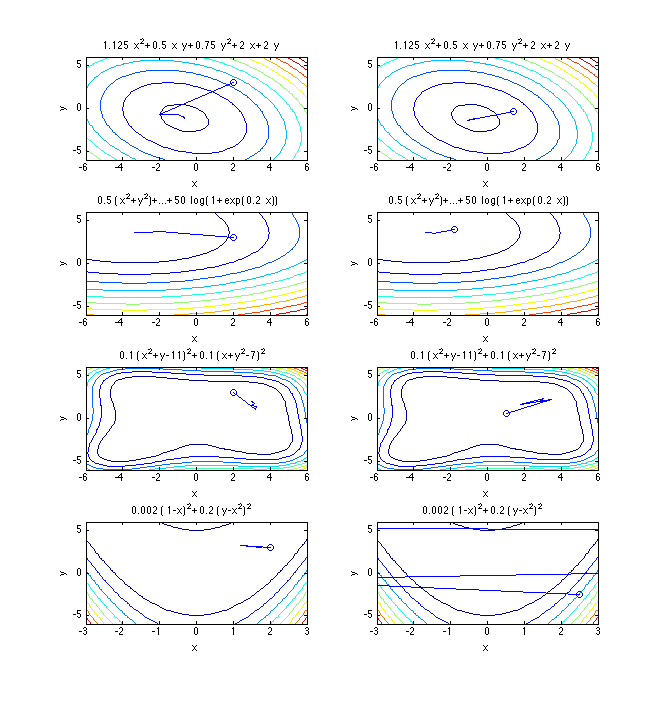
\includegraphics[width=1\textwidth]{img/gd_poly.png}}
       \caption{Gradient descent with $\frac{1}{k}$ step size: each row is a different
       function, the first column is with fixed initialization, and the second is with 
       random initialization.}
\end{figure}

\newpage
For some problems, the large step-size does not work. Firstly, if we examine
the eigenvalues of the hessian we see negative values (in the latter two
functions), which implies that these latter functions are not convex. Secondly,
a larger step-size corresponds with a higher Lipschitz constant (i.e. one needs
the step size to be bounded by $\frac{1}{L}$, where $L$ is the Lipschitz
coefficient), which might break whatever Lipschitz continuity assumption we are
making. Note that two sufficient conditions for the step sizes $\epsilon_t$ are
that
\begin{align}
    \sum_{t=1}^{\infty} \epsilon_t  &= \infty \\
    \sum_{t=1}^{\infty} \epsilon_t^{2} &< \infty
\end{align}


\end{document}
